\section{Verifying the Integrity of the Hosts  File}
\subsection{Activity}

\noindent {\bf{Bước 1:}} Truy cập vào đường dẫn \href{https://github.com/jessek/hashdeep/releases}{Link} rồi tải về file \textbf{md5deep\-4.4.zip}.

\begin{figure}[!htb]
    \centering
    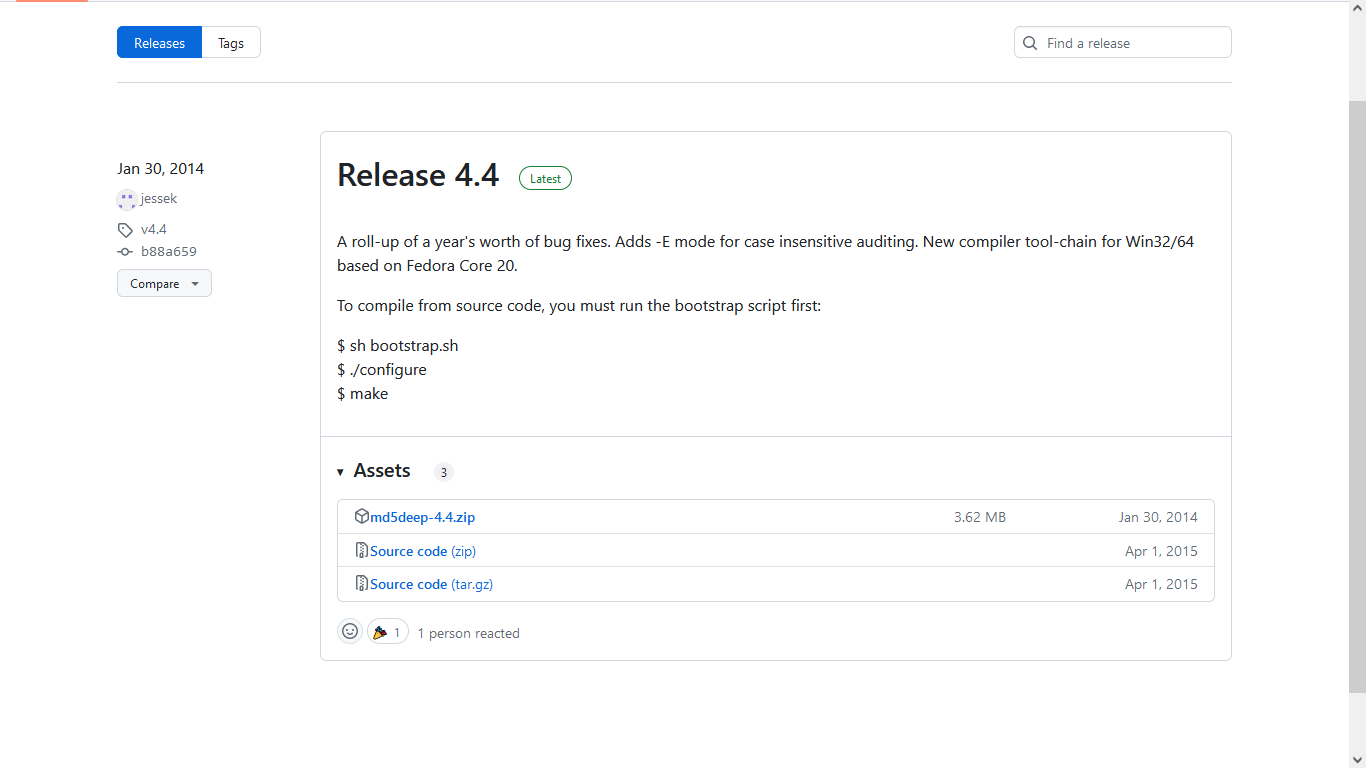
\includegraphics[width=1\linewidth]{figure//chapter9//lab9_1/hashdeep.png}
    \caption{Github của HashDeep}
    \label{fig:enter-label}
\end{figure}

\noindent {\bf{Bước 2:}} Giải nén file vào ổ C rồi lưu dưới tên là md5.

\begin{figure}[!htb]
    \centering
    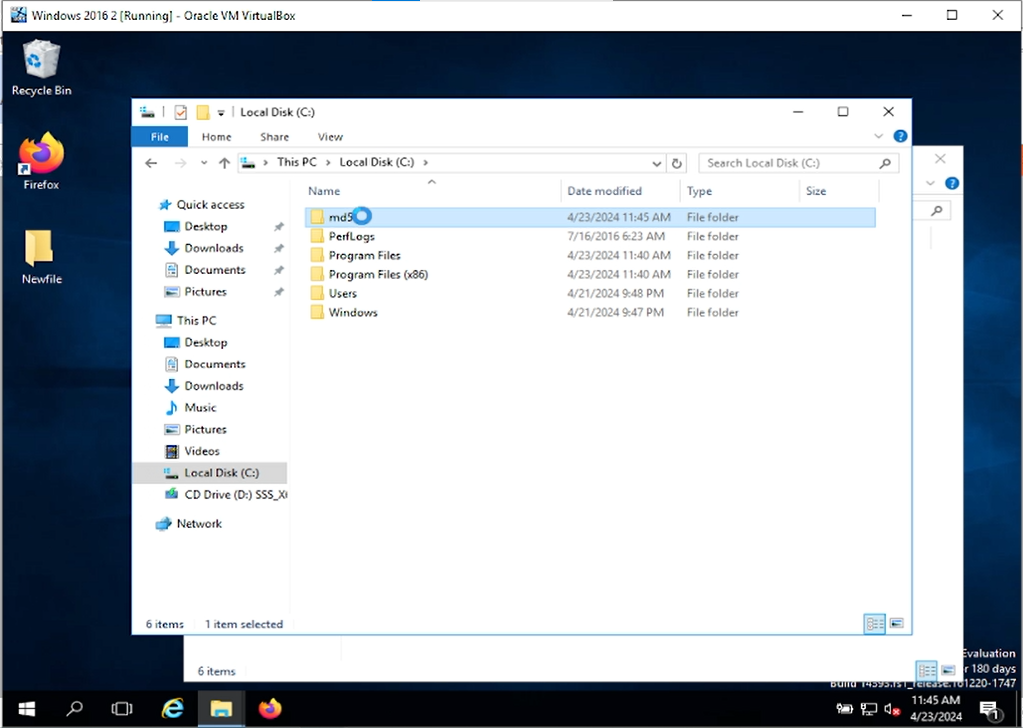
\includegraphics[width=0.9\linewidth]{figure//chapter9//lab9_1/extract.png}
    \caption{Kết quả sau khi giải nén}
    \label{fig:enter-label}
\end{figure}

\noindent {\bf{Bước 3:}} Mở \textbf{Notepad}, chọn \textbf{Open} và điều hướng tới C:>Windows>System32\\>drivers>etc. Chuyển loại file thành All Files. Sau đó chọn tệp \textbf{hosts}.

\begin{figure}[!htb]
    \centering
    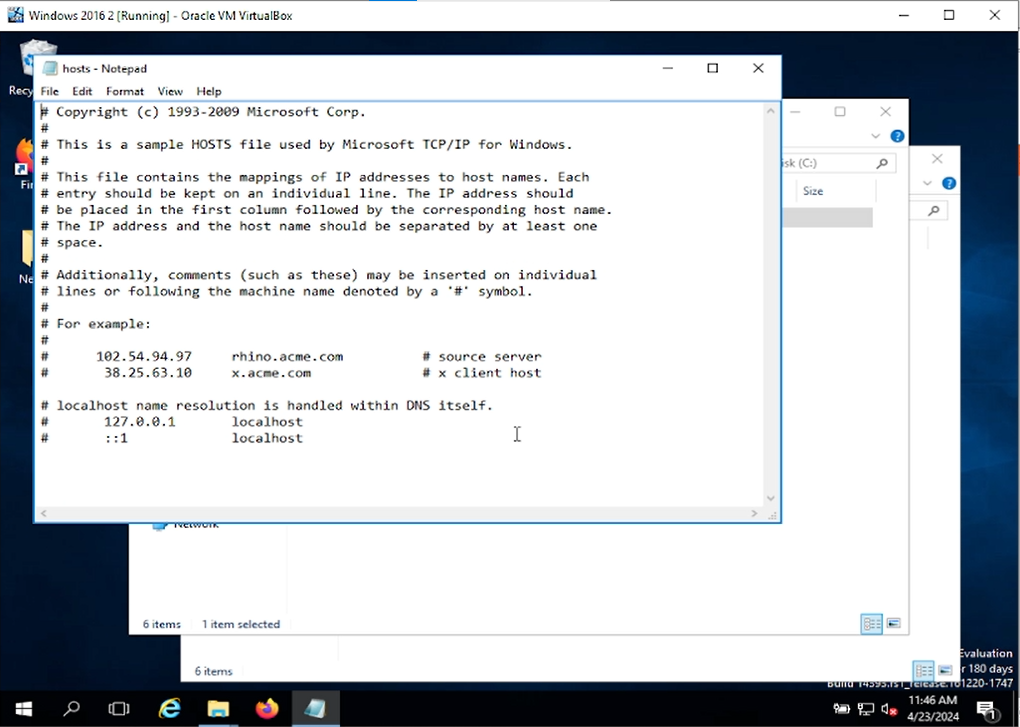
\includegraphics[width=0.8\linewidth]{figure//chapter9//lab9_1/hosts_file.png}
    \caption{Nội dung tệp hosts}
    \label{fig:enter-label}
\end{figure}

\noindent {\bf{Bước 4:}} Đóng tệp và mở \textbf{cmd}

\noindent {\bf{Bước 5:}} Điều hướng tới file \textbf{md5} vừa giải nén, sau đó nhập lệnh \textbf{dir}. Chú ý kết quả hiện ra 1 vài file .exe.

\begin{figure}[!htb]
    \centering
    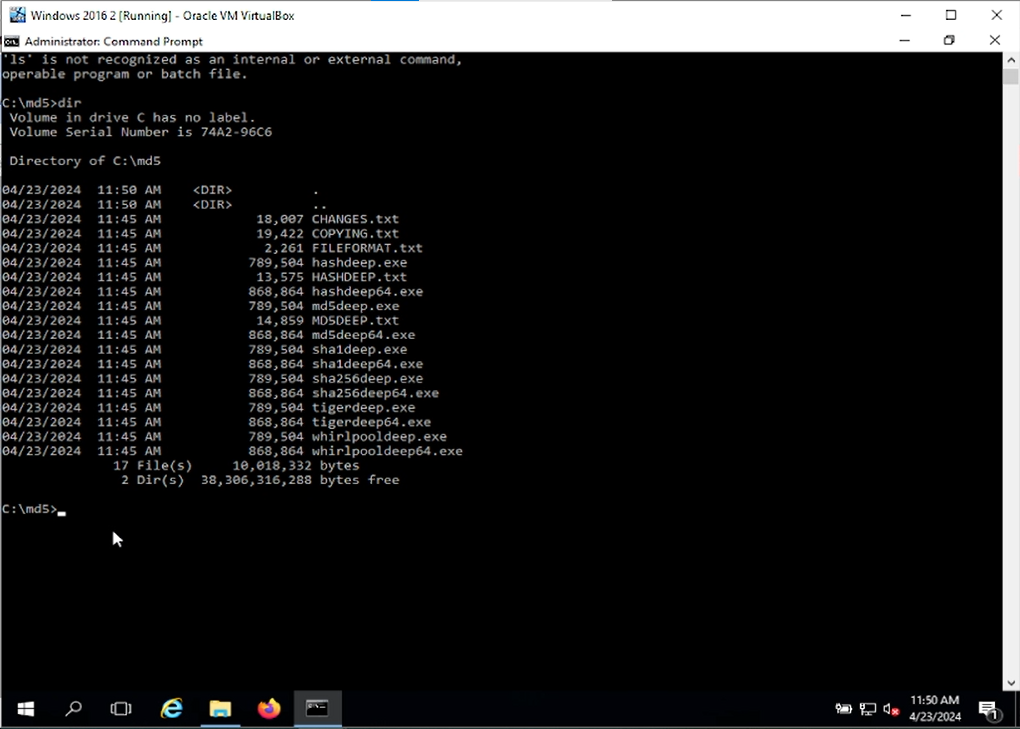
\includegraphics[width=0.85\linewidth]{figure//chapter9//lab9_1/dir_result.png}
    \caption{Kết quả khi chạy lệnh dir}
    \label{fig:enter-label}
\end{figure}

\newpage
\noindent {\bf{Bước 6:}} Thực hiện lệnh \textbf{sha256deep C:/Windows/Systems32/Drivers\\/hosts}. Kết quả nhận được một mã hash.

\begin{figure}[!htb]
    \centering
    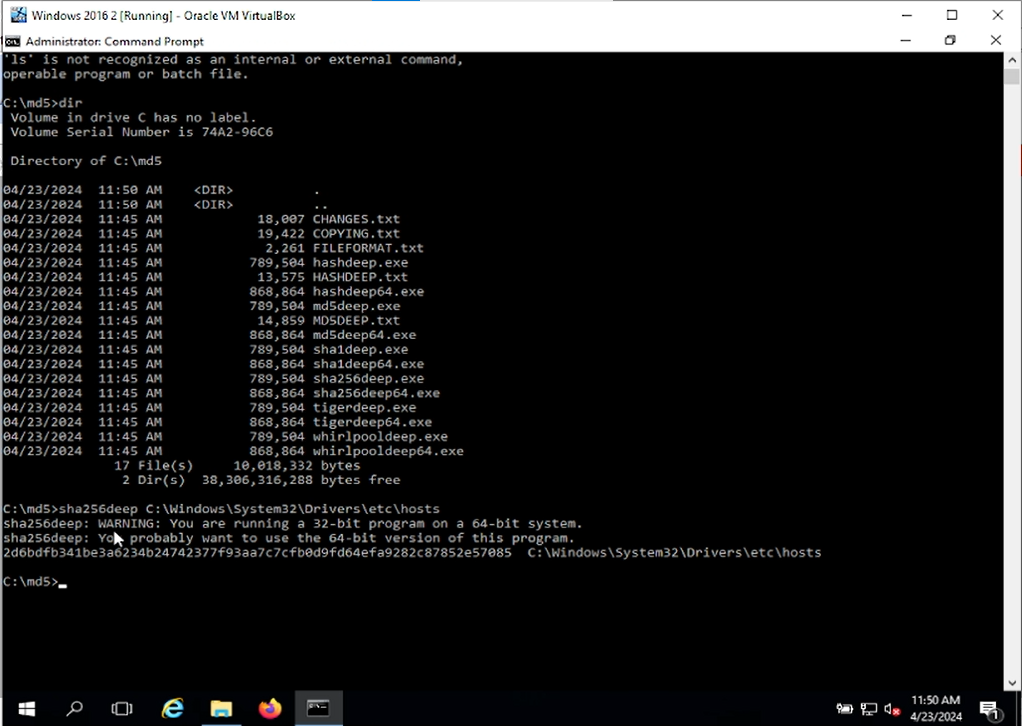
\includegraphics[width=0.85\linewidth]{figure//chapter9//lab9_1/hashcode.png}
    \caption{Hashcode nhận được sau khi thực hiện lệnh sha256deep}
    \label{fig:enter-label}
\end{figure}

\noindent {\bf{Bước 7:}} Copy mã hash đó vào trong Nodepad và lưu vào file có tên là \textbf{hosthash} rồi lưu ở \textbf{Desktop}.

\noindent {\bf{Bước 8:}} Mở lại tệp \textbf{hosts} ở bước trước đó. Thêm dòng sau vào cuối tệp: \textbf{69.32.133.79 www.boguswebaddress.net}. Sau đó lưu file lại.

\begin{figure}[!htb]
    \centering
    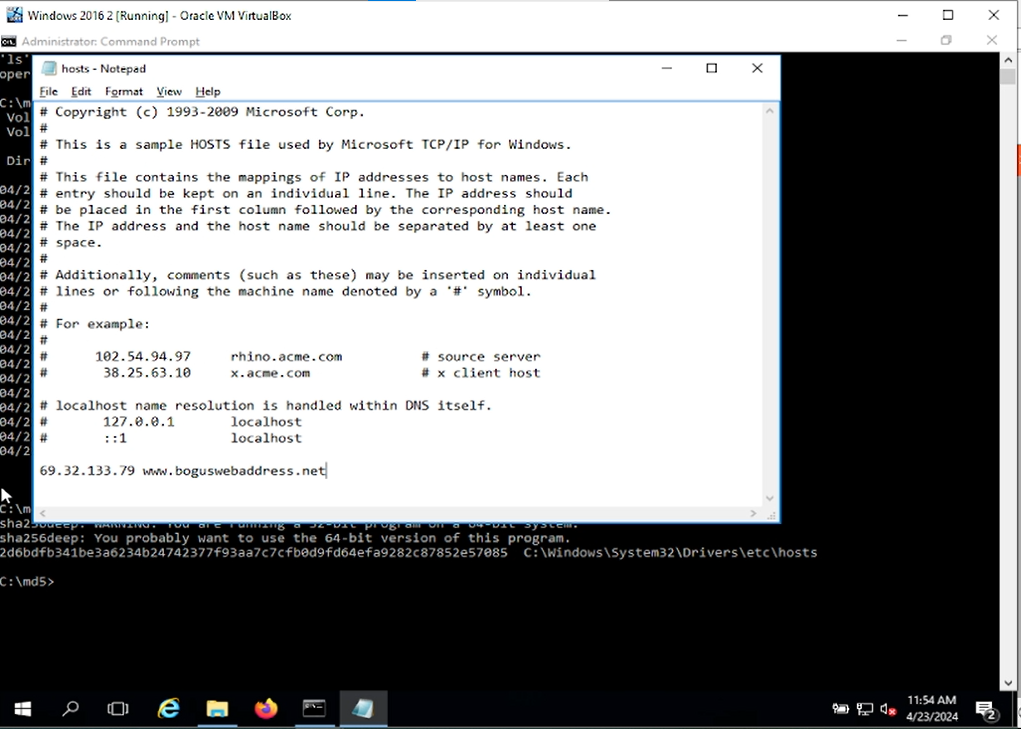
\includegraphics[width=0.8\linewidth]{figure//chapter9//lab9_1/edit.png}
    \caption{Chỉnh sửa tệp hosts}
    \label{fig:enter-label}
\end{figure}

\noindent {\bf{Bước 9:}} Thực hiện lại bước 6 và 7. Khi đó, 2 mã hash là khác nhau.

\begin{figure}[!htb]
    \centering
    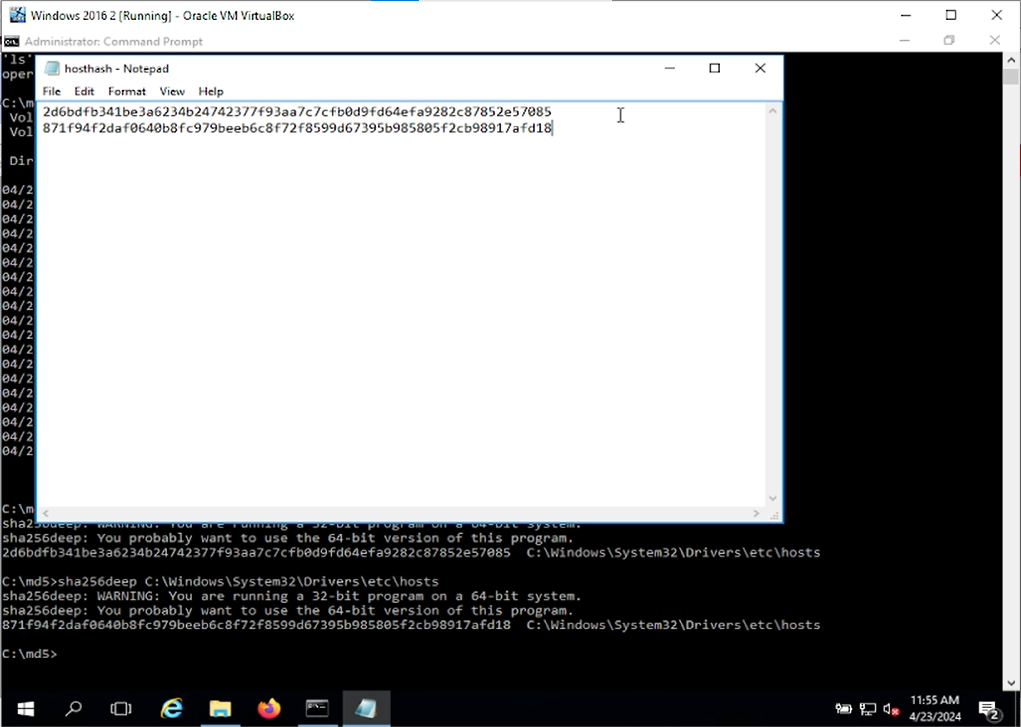
\includegraphics[width=0.85\linewidth]{figure//chapter9//lab9_1/diff-hash.png}
    \caption{Hai mã Hash khác nhau}
    \label{fig:enter-label}
\end{figure}

\noindent {\bf{Bước 10:}} Truy cập lại vào trang web được nhập vào tệp \textbf{hosts} thì không được.

\begin{figure}[!htb]
    \centering
    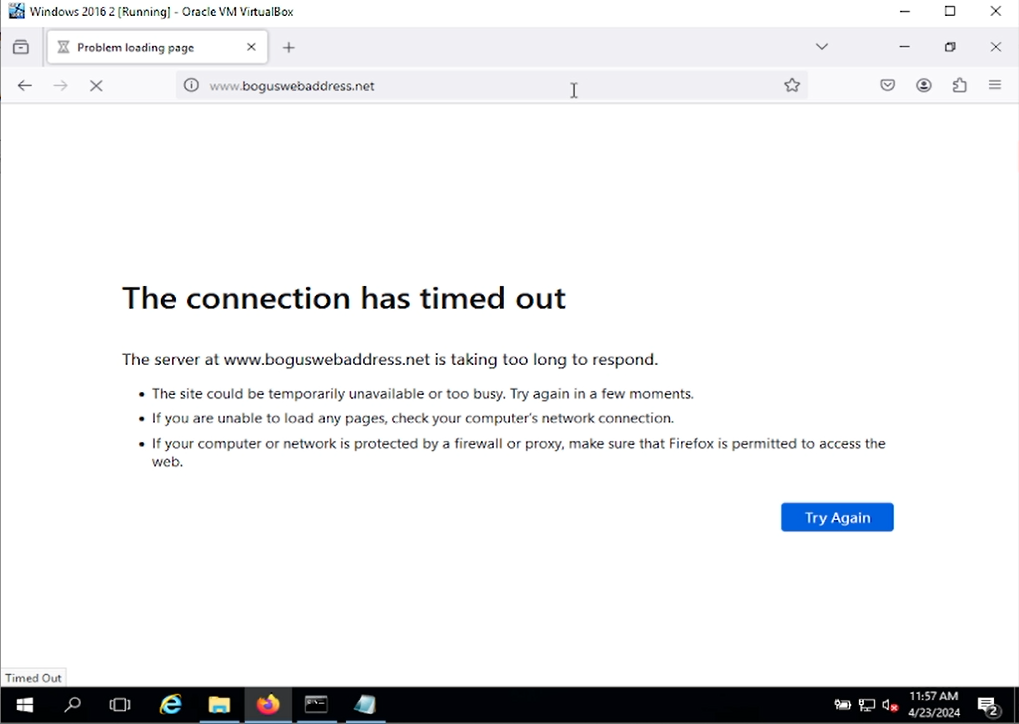
\includegraphics[width=0.8\linewidth]{figure//chapter9//lab9_1/failed-access.png}
    \caption{Không thể truy cập vào địa chỉ www.boguswebaddress.net}
    \label{fig:enter-label}
\end{figure}

\newpage

\subsection{Review Questions}

\noindent Câu 1:

C: AAAA.

\noindent Câu 2: 

D: ::1.

\noindent Câu 3: 

C: 64.

\noindent Câu 4: 

C: When a 200 MB file that has been previously hashed has one byte changed, a second hash of the file will be much less similar to the first hash than would be the case if the file had only been 200 KB in size.

\noindent Câu 5:

C: Prevention of unauthorized file modification.